The datasheet of a loudspeaker labelled ``\SI{8}{\ohm}'' shows its impedance against the frequency (measured, logarithmic frequency axis). The voice coil is a coil of wire, with a resistance $R$ and an inductance $L$, that sits in a magnet and drives the cone; the cone hangs on a soft suspension.

\begin{center}
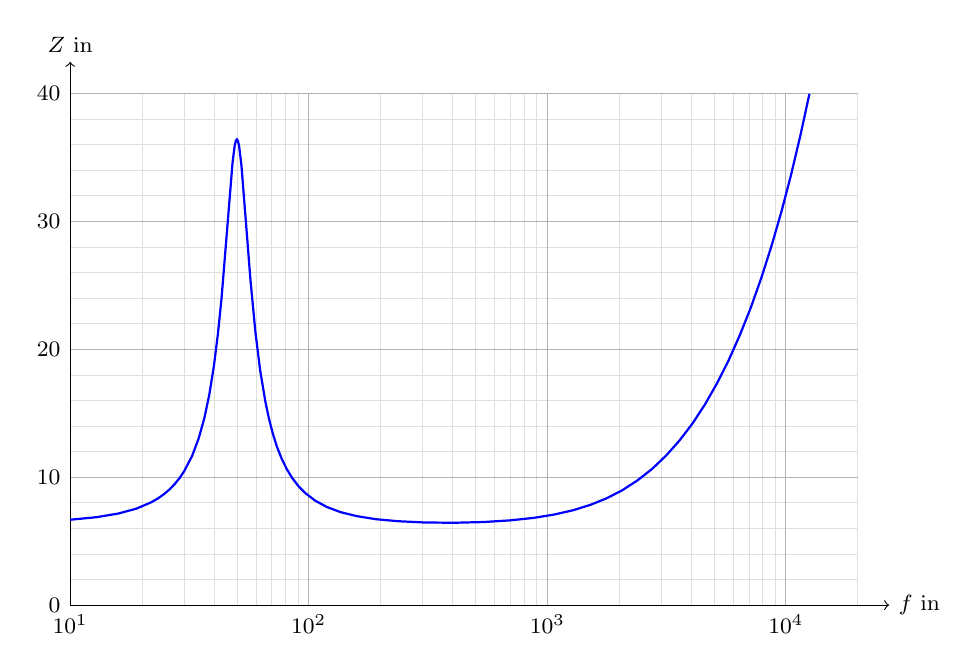
\begin{tikzpicture}[font=\footnotesize]
 \draw[gray!25, very thin] (0.912,0) -- (0.912,6.500) (1.445,0) -- (1.445,6.500) (1.824,0) -- (1.824,6.500) (2.117,0) -- (2.117,6.500) (2.357,0) -- (2.357,6.500) (2.560,0) -- (2.560,6.500) (2.736,0) -- (2.736,6.500) (2.891,0) -- (2.891,6.500) (3.941,0) -- (3.941,6.500) (4.475,0) -- (4.475,6.500) (4.853,0) -- (4.853,6.500) (5.147,0) -- (5.147,6.500) (5.387,0) -- (5.387,6.500) (5.589,0) -- (5.589,6.500) (5.765,0) -- (5.765,6.500) (5.920,0) -- (5.920,6.500) (6.971,0) -- (6.971,6.500) (7.504,0) -- (7.504,6.500) (7.883,0) -- (7.883,6.500) (8.176,0) -- (8.176,6.500) (8.416,0) -- (8.416,6.500) (8.619,0) -- (8.619,6.500) (8.794,0) -- (8.794,6.500) (8.949,0) -- (8.949,6.500) (10.000,0) -- (10.000,6.500);
 \draw[gray!25, very thin] (0,0.325) -- (10.000,0.325) (0,0.650) -- (10.000,0.650) (0,0.975) -- (10.000,0.975) (0,1.300) -- (10.000,1.300) (0,1.950) -- (10.000,1.950) (0,2.275) -- (10.000,2.275) (0,2.600) -- (10.000,2.600) (0,2.925) -- (10.000,2.925) (0,3.575) -- (10.000,3.575) (0,3.900) -- (10.000,3.900) (0,4.225) -- (10.000,4.225) (0,4.550) -- (10.000,4.550) (0,5.200) -- (10.000,5.200) (0,5.525) -- (10.000,5.525) (0,5.850) -- (10.000,5.850) (0,6.175) -- (10.000,6.175);
 \draw[gray!60, thin] (0.000,0) -- (0.000,6.500) (3.029,0) -- (3.029,6.500) (6.059,0) -- (6.059,6.500) (9.088,0) -- (9.088,6.500);
 \draw[gray!60, thin] (0,0.000) -- (10.000,0.000) (0,1.625) -- (10.000,1.625) (0,3.250) -- (10.000,3.250) (0,4.875) -- (10.000,4.875) (0,6.500) -- (10.000,6.500);
 \node[below] at (0.000,0) {$10^{1}$};
 \node[below] at (3.029,0) {$10^{2}$};
 \node[below] at (6.059,0) {$10^{3}$};
 \node[below] at (9.088,0) {$10^{4}$};
 \node[left] at (0,0.000) {0};
 \node[left] at (0,1.625) {10};
 \node[left] at (0,3.250) {20};
 \node[left] at (0,4.875) {30};
 \node[left] at (0,6.500) {40};
 \draw[->] (0,0) -- (10.400,0) node[right] {$f$ in \si{\hertz}};
 \draw[->] (0,0) -- (0,6.900) node[above] {$Z$ in \si{\ohm}};
 \draw[thick, blue] plot coordinates {(0.000,1.084) (0.337,1.117) (0.612,1.163) (0.840,1.225) (1.030,1.306) (1.115,1.355) (1.192,1.410) (1.264,1.471) (1.330,1.541) (1.390,1.615) (1.447,1.700) (1.549,1.896) (1.630,2.112) (1.704,2.375) (1.767,2.675) (1.825,3.037) (1.875,3.435) (1.922,3.896) (2.062,5.621) (2.090,5.842) (2.104,5.897) (2.117,5.915) (2.130,5.896) (2.145,5.831) (2.175,5.582) (2.290,4.122) (2.352,3.469) (2.412,2.984) (2.479,2.581) (2.524,2.369) (2.572,2.182) (2.625,2.013) (2.684,1.864) (2.749,1.730) (2.819,1.615) (2.897,1.513) (2.982,1.426) (3.112,1.326) (3.262,1.245) (3.436,1.180) (3.639,1.130) (3.882,1.091) (4.169,1.065) (4.509,1.049) (4.884,1.046) (5.249,1.055) (5.584,1.076) (5.881,1.107) (6.146,1.150) (6.388,1.205) (6.609,1.274) (6.816,1.358) (7.010,1.458) (7.206,1.585) (7.393,1.732) (7.571,1.902) (7.741,2.094) (7.905,2.309) (8.063,2.551) (8.216,2.819) (8.363,3.111) (8.506,3.433) (8.645,3.782) (8.778,4.158) (8.908,4.566) (9.033,4.999) (9.155,5.465) (9.273,5.963) (9.388,6.492)};
\end{tikzpicture}
\end{center}

\begin{abcliste}
\abc What is the resistance $R$ of the voice coil?
\abc At which frequency $f_s$ does the cone resonate on its suspension?
\abc At high frequencies, the inductance of the voice coil makes $Z$ rise. Find $L$ from $Z$ at \faO.
\end{abcliste}
